\tikzstyle{block} = [draw, rectangle, minimum height=2.5em, minimum width=2.8em]
\tikzstyle{sum} = [draw, circle, node distance=0]
\tikzstyle{input} = [coordinate]
\tikzstyle{output} = [coordinate]
\tikzstyle{junction} =[circle,inner sep=1pt,minimum size=0.1mm,fill=black,draw=black]

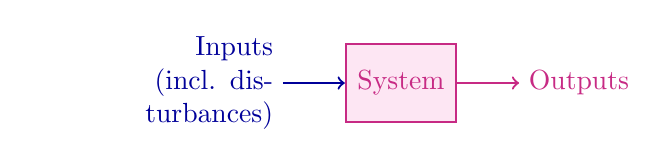
\begin{tikzpicture} [auto, node distance=2cm]

\def\colC{green!40!black};
\def\fillC{green!20!white};

\def\colS{magenta!80!black};
\def\fillS{magenta!10!white};

\def\colE{blue!60!black};
\def\fillE{cyan!20!white};

\node at (0,0)[block,thick,
               draw=\colS,fill=\fillS,
               minimum width=1.4cm,minimum height=1cm]
               (S) {\textcolor{\colS}{System}};

\node[block,left of=S,align=right,
      draw=none,fill=none,text width=3cm,
      node distance=1.5cm,anchor=east]
      (U) {\textcolor{\colE}
          {Inputs\\(incl. disturbances)}};

\draw[->,thick,\colE]
      (U.east) -- (S.west);

\node[right of=S,anchor=west,
      node distance=1.5cm]
      (Y) {\textcolor{\colS}{Outputs}};

\draw[->,thick,\colS]
      (S.east) -- (Y.west);

\end{tikzpicture}
